% \bibliography{../src/bibliography.bib}

% In this appendix we give an account of variational inference in general of amortized variational inference in particular. We focus on amortized inference with discrete latent variables, and in particular when the variables are structured. We then derive the score function gradient, as used in chapter \ref{05-semisupervised}, and we describe techniques to reduce the variance of this estimator.


% \section{Variational Inference}
% We will write some generic things about variational inference.
% \begin{itemize}
%   \item Variational inference for exponential families, with conjugate priors \citep{jordan1999vi,jordan2008graphical,blei2016vi}.
%   \item With amortized inference, using neural networks, for non-conjugate models \citep{kingma2014vae,rezende2014dgm} and in particular the reparametrization trick that makes these models efficiently trainable.
%   \item Reparametrization for discrete latent variables \citep{maddison2017concrete,jang2017gumbel}.
%   \item The generalization of this reparametrization trick in automatic differentiation variational inference \citep{kucukelbir2017automatic}.
%   \item Black box variational inference, which uses the same combination of score function gradient with variance reduction that we resort to \citep{ranganath2014black}.
% \end{itemize}


\section{Derivation}
This section provides detailed derivation of the score function estimator:
\begin{align}
  \label{eq:score-function-estimator}
  \nabla_{\lambda} \expect_{q} [ L(\x, \y) ] = \expect_{q} [ L(\x, \y) \nabla_{\lambda} \log \qlambda(\y | \x) ]
\end{align}
where
\begin{equation*}
  L(\x, \y) \defeq \log \ptheta(\x, \y) - \log \qlambda(\y | \x).
\end{equation*}
The line by line derivation:
\begin{align*}
  \nabla_{\lambda} \expect_{q} [ L(\x, \y) ] &=
  \nabla_{\lambda} \expect_{q} [ \log \ptheta(\x, \y) - \log \qlambda(\y | \x) ] \\
    &= \nabla_{\lambda} \sum_{\y \in \yieldx} \Big\{ \qlambda(\y | \x) \log \ptheta(\x, \y) - \qlambda(\y | \x)\log \qlambda(\y | \x) \Big\} \\
    &= \sum_{\y \in \yieldx} \Big\{ \nabla_{\lambda} \qlambda(\y | \x) \log \ptheta(\x, \y)  - \nabla_{\lambda} \qlambda(\y | \x)\log \qlambda(\y | \x) \\
    &\qquad -  \qlambda(\y | \x)\nabla_{\lambda}\log \qlambda(\y | \x) \Big\} \\
    &= \sum_{\y \in \yieldx} \Big\{ \nabla_{\lambda} \qlambda(\y | \x) \log \ptheta(\x, \y) - \nabla_{\lambda} \qlambda(\y | \x)\log \qlambda(\y | \x) \Big\} \\
    &= \sum_{\y \in \yieldx} \Big\{ L(\x, \y)\nabla_{\lambda} \qlambda(\y | \x) \Big\} \\
    &= \sum_{\y \in \yieldx} \Big\{ L(\x, \y) \qlambda(\y | \x) \nabla_{\lambda} \log \qlambda(\y | \x) \Big\}   \\
    &= \expect_{q} \Big[ L(\x, \y) \nabla_{\lambda} \log \qlambda(\y | \x) \Big].
\end{align*}
In this derivation we used the identity
\begin{align*}
  \nabla_{\lambda} \qlambda(\y | \x) &= \qlambda(\y | \x)\nabla_{\lambda}\log \qlambda(\y | \x),
\end{align*}
which follows from the derivative
\begin{align*}
  \nabla_{\lambda}\log \qlambda(\y | \x) &= \nabla_{\lambda} \qlambda(\y | \x)\qlambda(\y | \x)^{-1},
\end{align*}
and finally the fact that
\begin{align*}
  \sum_{\y \in \yieldx} \qlambda(\y | \x)\nabla_{\lambda}\log \qlambda(\y | \x)
    &= \sum_{\y \in \yieldx}  \qlambda(\y | \x) \frac{\nabla_{\lambda} \qlambda(\y | \x)}{\qlambda(\y | \x)}  \\
    &= \sum_{\y \in \yieldx} \nabla_{\lambda} \qlambda(\y | \x) \\
    &= \nabla_{\lambda} \sum_{\y \in \yieldx} \qlambda(\y | \x)\\
    &= \nabla_{\lambda} 1 \\
    &= 0. \\
\end{align*}


\section{Optimization}
We use automatic differentiation \citep{baydin2017automatic} to obtain all our gradients. In order to obtain the gradients in formula \ref{eq:score-function-estimator} using this method we rewrite it in the form of a \textit{surrogate objective} \citep{schulman2015gradient}:
\begin{align}
  \label{eq:surrogate}
  \objective_{ \textsc{surr} }(\theta, \lambda) &= \frac{1}{K}\sum_{i=1}^K \log \qlambda(\x | \y_i) \blockgrad( L(\x, \y_i) ).
\end{align}
The function $\blockgrad$ detaches a node from its upstream computation graph. This turns it effectively into a scalar. To roughly illustrate this, let $f$ be function (computed by a node in the computation graph) with parameters $\theta$ and input $\x$, then
\begin{align*}
  \blockgrad(f_{\theta}( \x )) &\defeq f( \x ),
\end{align*}
such that
\begin{align*}
  \nabla_{\theta}\blockgrad(f_{\theta}( \x )) = \nabla_{\theta} f( \x ) = 0.
\end{align*}
Automatic differentiation of equation \ref{eq:surrogate} with respect to $\lambda$ will give us the exact expression we are looking for
\begin{align*}
  \nabla_{\lambda} \objective_{ \textsc{surr} }(\theta, \lambda) &= \frac{1}{K}\sum_{i=1}^K L(\x, \y) \nabla_{\lambda} \log\qlambda( \x | \y_i ),
\end{align*}
hence the adjective \textit{surrogate}.

\section{Variance reduction}
We have derived an estimator for the gradient of the posterior parameters in the unsupervised objective. This estimator is unbiased, but is known to have high variance, often too much to be useful \citep{paisley2012viss}. Two effective methods to counter this are control variates and baselines \citep{ross2006simulation}.

\subsection{Variance}
Our expectation is of the general form
\begin{align*}
  \mu \defeq \expect [ f(X) ]
\end{align*}
and that we estimate this quantity by generating $n$ independent samples $X_1,\dots,X_n \sim P(X)$ and computing
\begin{align*}
  \hat{\mu} \defeq \frac{1}{n} \sum_{i=1}^n f(X_i).
\end{align*}
% This is an unbiased estimator for $\mu$ with error
% \begin{align*}
%   \Big[(\mu - \hat{\mu})^2 \Big] &= \var \Big[ \hat{\mu} \Big] = \frac{\var \Big[ \hat{\mu} \Big]}{n},
% \end{align*}
% which means that the error
% \begin{align*}
%   \mu - \hat{\mu} = O \Bigg( \sqrt{\frac{\var \Big[ \hat{\mu} \Big] }{n}} \Bigg)
% \end{align*}
% and reducing it linearly requires a quadratic number of samples.
In our particular case, the function $f$ is
\begin{equation*}
  f(Y) \defeq L(x,Y) \nabla_{\lambda} \log q_{\lambda}(Y|X=x)
\end{equation*}
where we have made explicit that $y$ is the random variable, and $x$ is given.

\subsection{Control variates}
Consider a function $g$ with known expectation
\begin{align*}
  \mu_{g} \defeq \expect [ g(X) ].
\end{align*}
Then we can define a new function $\hat{f}$ such that
\begin{align*}
  \hat{f}(X) \defeq f(X) - g(X) + \mu_{g}.
\end{align*}
This function is also an estimator for $\mu$, since
\begin{align*}
    \expect [ \hat{f}(X) ] &= \expect [ f(X) ] - \mu_{g} + \mu_{g} \\
        &= \expect [ f(X) ],
\end{align*}
and a computation shows that the variance of the new function is
\begin{align*}
  \var [ \hat{f}(X) ]
    &= \expect [ (f(X) - g(X) + \mu_{g}) - \mu)^2 ] \\
    &= \expect [ (f(X) - g(X) + \mu_{g})^2 ] - 2\expect [ (f(X) - g(X) + \mu_{g})\mu ] \\
    &\quad+ \expect [ \mu^2 ] \\
    &= \expect [ (f(X) - g(X) + \mu_{g})^2 ] - 2\expect [ (f(X) - g(X) + \mu_{g})]\mu + \mu^2 \\
    &= \expect [ (f(X) - g(X) + \mu_{g})^2 ] - 2\mu^2  + \mu^2 \\
    &= \expect [ f(X)^2 + g(X)^2 + \mu_{g}^2 - 2f(X)g(X) + 2f(X)\mu_{g} - 2g(X)\mu_{g} ] \\
    &\quad- \mu^2\\
    &= \expect [ f(X)^2 ] - \expect [ f(X) ]^2 \\
      &\quad - 2(\expect [ f(X)g(X) ] - \expect [ f(X) ]\expect [ g(X) ]) \\
      &\quad + \expect [ g(X)^2 ] - \expect [ g(X) ]^2 \\
    &= \var [ f(X) ] - 2  \cov [ f(X), g(X) ] + \var [ g(X) ]
\end{align*}
This means we can get a reduction in variance whenever
\begin{equation*}
  \cov [ f(X), g(X) ] > \frac{1}{2} \var [ g(X) ].
\end{equation*}
The function $g$ is called a \textit{control variate}---it allows us to control the variance of $f$.

From the equality above we can see that this will be the case whenever $f(X)$ and $g(X)$ are strongly correlated. Our choice of control variate will be made with the that in mind. Furthermore, $\expect [ g(X) ]$ must be known. What is an optimal control variate? Typically a control variate of the form $ag$ is chosen with fixed, and $a$ is optimized to maximize the correlation. This brings us to the generic formulation of a control variate:
\begin{align*}
    \hat{f}(X) \defeq f(X) - a(g(X) - \expect [ g(X) ])
\end{align*}
with variance
\begin{align*}
  \var [ \hat{f}(X) ] = \var [ f(X) ] - 2a  \cov [ f(X), g(X) ] + a^2 \var [ g(X) ]
\end{align*}
We take a derivative of this with respect to $a$
\begin{align*}
    \frac{d}{d a}\var [ \hat{f}(X) ] &= - 2  \cov [ f(X), g(X) ] + 2a \var [ g(X) ]
\end{align*}
Setting this to zero and solving for $a$ we obtain the optimal choice for $a$
\begin{align}
\label{eq:cv-scale}
  a &= \frac{ \cov [ f(X), g(X) ]}{ \var [ g(X) ]}.
\end{align}

Plugging in this solution into the expression for $\var [ \hat{f}(X) ]$ and dividing by $\var [ f(X) ]$ we get
\begin{align}
\label{eq:var-red}
  \frac{\var [ \hat{f}(X) ]}{\var [ f(X) ]}
    &= 1 - \frac{\cov[ f(X), g(X) ]}{ \var [ f(X) ]  \var [ g(X) ]} \\
    &= 1 - \corr^2 [ f(X), g(X) ],
\end{align}
which shows that given this choice of $a$ the reduction in variance is directly determined by the correlation between $f(X)$ and $g(X)$.

Bringing this all together, we let our new estimator be
\begin{align*}
  \expect [ f(X) ]
    &= \expect [ \hat{f}(X) ] \approx \frac{1}{n} \sum_{i=1}^n [ f(X_i) - ag(X_i) ] - \mu_{g}
\end{align*}

\begin{example}{\citep{ross2006simulation}}
  Suppose we want to use simulation to determine
  \begin{equation*}
      \expect [ f(X) ] = \expect [ e^X ] = \int_0^1 e^x dx = e - 1
  \end{equation*}
  with $X \sim \text{Uniform}(0,1)$. A natural control variate to use in this case is the random variable $X$ itself: $g(X) \defeq X$. We thus define the new estimator
  \begin{align*}
    \hat{f}(X)
      &= f(X) - g(X) + \expect [ g(X) ]  \\
      &= e^X - X + \frac{1}{2}.
  \end{align*}

  To compute the decrease in variance with this new estimator, we first note that
  \begin{align*}
    \cov(e^X, X)
      &= \expect [ Xe^X ] - \expect [ X ]\expect [ e^X ] \\
      &= \int_0^1 xe^x dx - \frac{e-1}{2} \\
      &= 1 - \frac{e-1}{2} \approx 0.14086 \\
    \var [ e^X ]
      &= \expect [ e^{2X} ] - (\expect [ e^X ])^2 \\
      &= \int_0^1 e^{2x} dx - (1 - e^x)^2 \\
      &= \frac{e^2 - 1}{2}  - (1 - e^x)^2 \approx 0.2420 \\
    \var [ X ] &= \expect [ X^2 ] - (\expect [ X ])^2 \\
      &= \int_0^1 x^2 dx - \frac{1}{4} \\
      &= \frac{1}{3} - \frac{1}{4} = \frac{1}{12}.
  \end{align*}
  When we choose $a$ as in formula \ref{eq:cv-scale} we can use formula \ref{eq:var-red} to compute that
  \begin{align*}
    \frac{ \var [ \hat{f}(X) ] }{ \var [ f(X) ]}
      &= 1 - \frac{(0.14086)^2}{\frac{0.2420}{12}} \\
      &\approx 0.0161.
  \end{align*}
  This is a reduction of 98.4 percent!

% A simulation illustrates what this looks like in practice with \dots samples:
%   \begin{figure}
%     \center
%     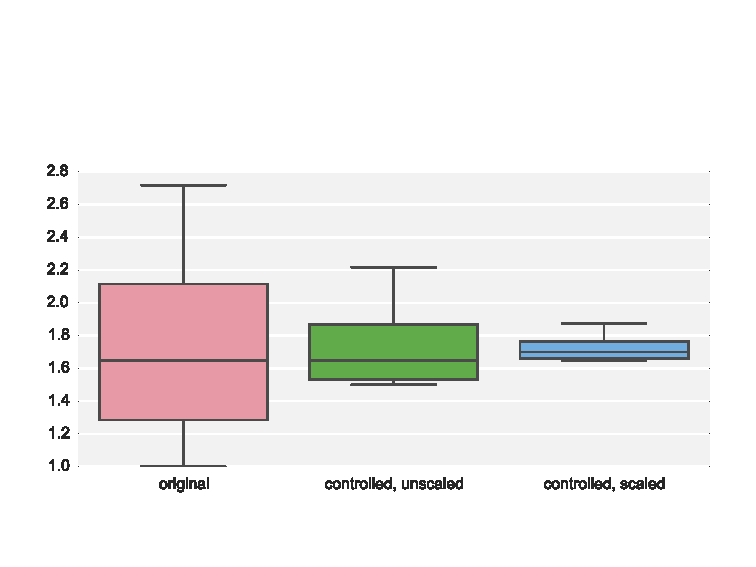
\includegraphics[width=0.7\textwidth]{control-variate.pdf}
%   \end{figure}
% \end{example}
